\documentclass{standalone}
\usepackage{tikz}
\usetikzlibrary{patterns, positioning}


\begin{document}
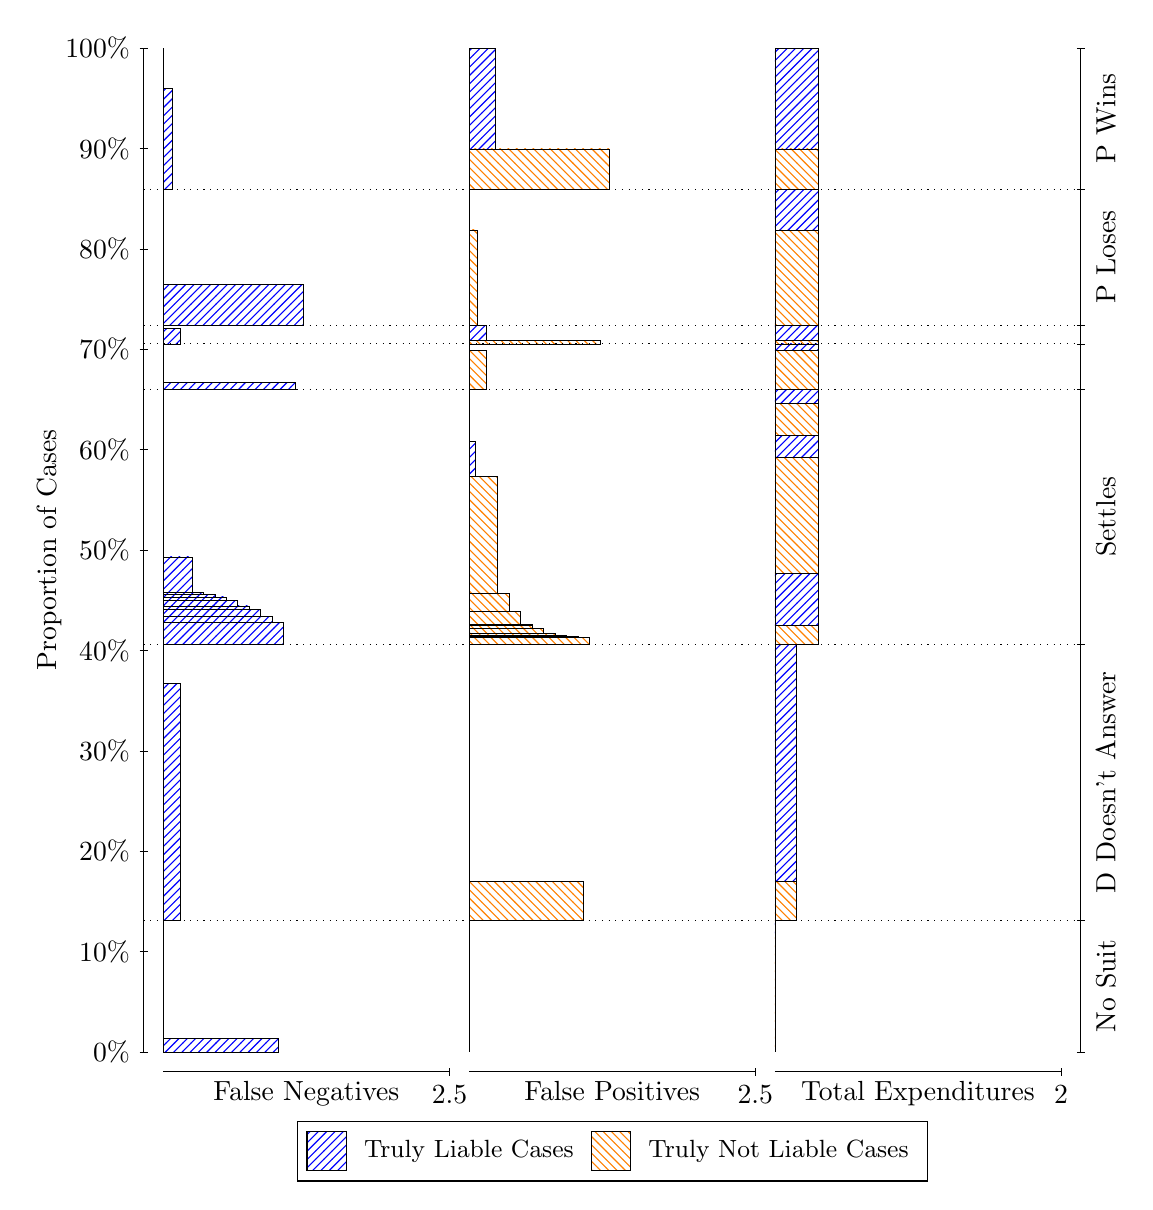
\begin{tikzpicture}
\draw[black, very thin] (1.5,1.75) -- (1.5,14.5);
\node[rotate=90, text=black, anchor=center] at (0.3, 8.125) {Proportion of Cases};
\draw[black, very thin] (1.45,1.75) -- (1.55,1.75);
\node[text=black, anchor=east] at (1.45, 1.75) {0\%};
\draw[black, very thin] (1.45,3.025) -- (1.55,3.025);
\node[text=black, anchor=east] at (1.45, 3.025) {10\%};
\draw[black, very thin] (1.45,4.3) -- (1.55,4.3);
\node[text=black, anchor=east] at (1.45, 4.3) {20\%};
\draw[black, very thin] (1.45,5.575) -- (1.55,5.575);
\node[text=black, anchor=east] at (1.45, 5.575) {30\%};
\draw[black, very thin] (1.45,6.85) -- (1.55,6.85);
\node[text=black, anchor=east] at (1.45, 6.85) {40\%};
\draw[black, very thin] (1.45,8.125) -- (1.55,8.125);
\node[text=black, anchor=east] at (1.45, 8.125) {50\%};
\draw[black, very thin] (1.45,9.4) -- (1.55,9.4);
\node[text=black, anchor=east] at (1.45, 9.4) {60\%};
\draw[black, very thin] (1.45,10.675) -- (1.55,10.675);
\node[text=black, anchor=east] at (1.45, 10.675) {70\%};
\draw[black, very thin] (1.45,11.95) -- (1.55,11.95);
\node[text=black, anchor=east] at (1.45, 11.95) {80\%};
\draw[black, very thin] (1.45,13.225) -- (1.55,13.225);
\node[text=black, anchor=east] at (1.45, 13.225) {90\%};
\draw[black, very thin] (1.45,14.5) -- (1.55,14.5);
\node[text=black, anchor=east] at (1.45, 14.5) {100\%};

\draw[black, very thin] (13.4,1.75) -- (13.4,14.5);
\draw[black, very thin] (13.35,1.75) -- (13.45,1.75);
\node[anchor=west] at (13.35, 1.75) {};
\draw[black, very thin] (13.35,3.4238) -- (13.45,3.4238);
\node[anchor=west] at (13.35, 3.4238) {};
\draw[black, very thin] (13.35,6.9296) -- (13.45,6.9296);
\node[anchor=west] at (13.35, 6.9296) {};
\draw[black, very thin] (13.35,10.166) -- (13.45,10.166);
\node[anchor=west] at (13.35, 10.166) {};
\draw[black, very thin] (13.35,10.742) -- (13.45,10.742);
\node[anchor=west] at (13.35, 10.742) {};
\draw[black, very thin] (13.35,10.98) -- (13.45,10.98);
\node[anchor=west] at (13.35, 10.98) {};
\draw[black, very thin] (13.35,12.704) -- (13.45,12.704);
\node[anchor=west] at (13.35, 12.704) {};
\draw[black, very thin] (13.35,14.5) -- (13.45,14.5);
\node[anchor=west] at (13.35, 14.5) {};

\draw[black, very thin, pattern color=blue, pattern=north east lines] (1.75,1.75) rectangle (3.2033,1.9261);
\draw[black, very thin, pattern color=orange, pattern=north west lines] (1.75,1.9261) rectangle (1.75,3.4238);
\draw[black, very thin, pattern color=blue, pattern=north east lines] (1.75,3.4238) rectangle (1.968,6.4348);
\draw[black, very thin, pattern color=orange, pattern=north west lines] (1.75,6.4348) rectangle (1.75,6.9296);
\draw[black, very thin, pattern color=blue, pattern=north east lines] (1.75,6.9296) rectangle (3.276,7.2062);
\draw[black, very thin, pattern color=blue, pattern=north east lines] (1.75,7.2062) rectangle (3.1307,7.2779);
\draw[black, very thin, pattern color=blue, pattern=north east lines] (1.75,7.2779) rectangle (2.9853,7.3716);
\draw[black, very thin, pattern color=blue, pattern=north east lines] (1.75,7.3716) rectangle (2.84,7.4158);
\draw[black, very thin, pattern color=blue, pattern=north east lines] (1.75,7.4158) rectangle (2.6947,7.4864);
\draw[black, very thin, pattern color=blue, pattern=north east lines] (1.75,7.4864) rectangle (2.5493,7.53);
\draw[black, very thin, pattern color=blue, pattern=north east lines] (1.75,7.53) rectangle (2.404,7.566);
\draw[black, very thin, pattern color=blue, pattern=north east lines] (1.75,7.566) rectangle (2.2587,7.589);
\draw[black, very thin, pattern color=blue, pattern=north east lines] (1.75,7.589) rectangle (2.1133,8.0377);
\draw[black, very thin, pattern color=orange, pattern=north west lines] (1.75,8.0377) rectangle (1.75,10.166);
\draw[black, very thin, pattern color=blue, pattern=north east lines] (1.75,10.166) rectangle (3.4213,10.252);
\draw[black, very thin, pattern color=orange, pattern=north west lines] (1.75,10.252) rectangle (1.75,10.742);
\draw[black, very thin, pattern color=blue, pattern=north east lines] (1.75,10.742) rectangle (1.968,10.939);
\draw[black, very thin, pattern color=orange, pattern=north west lines] (1.75,10.939) rectangle (1.75,10.98);
\draw[black, very thin, pattern color=blue, pattern=north east lines] (1.75,10.98) rectangle (3.5303,11.494);
\draw[black, very thin, pattern color=orange, pattern=north west lines] (1.75,11.494) rectangle (1.75,12.704);
\draw[black, very thin, pattern color=blue, pattern=north east lines] (1.75,12.704) rectangle (1.859,13.986);
\draw[black, very thin, pattern color=orange, pattern=north west lines] (1.75,13.986) rectangle (1.75,14.5);
\draw[black, very thin, pattern color=orange, pattern=north west lines] (5.6333,1.75) rectangle (5.6333,3.2477);
\draw[black, very thin, pattern color=blue, pattern=north east lines] (5.6333,3.2477) rectangle (5.6333,3.4238);
\draw[black, very thin, pattern color=orange, pattern=north west lines] (5.6333,3.4238) rectangle (7.0867,3.9186);
\draw[black, very thin, pattern color=blue, pattern=north east lines] (5.6333,3.9186) rectangle (5.6333,6.9296);
\draw[black, very thin, pattern color=orange, pattern=north west lines] (5.6333,6.9296) rectangle (7.1593,7.0116);
\draw[black, very thin, pattern color=orange, pattern=north west lines] (5.6333,7.0116) rectangle (7.014,7.0234);
\draw[black, very thin, pattern color=orange, pattern=north west lines] (5.6333,7.0234) rectangle (6.8687,7.0414);
\draw[black, very thin, pattern color=orange, pattern=north west lines] (5.6333,7.0414) rectangle (6.7233,7.064);
\draw[black, very thin, pattern color=orange, pattern=north west lines] (5.6333,7.064) rectangle (6.578,7.1309);
\draw[black, very thin, pattern color=orange, pattern=north west lines] (5.6333,7.1309) rectangle (6.4327,7.1687);
\draw[black, very thin, pattern color=orange, pattern=north west lines] (5.6333,7.1687) rectangle (6.4327,7.1778);
\draw[black, very thin, pattern color=orange, pattern=north west lines] (5.6333,7.1778) rectangle (6.2873,7.3495);
\draw[black, very thin, pattern color=orange, pattern=north west lines] (5.6333,7.3495) rectangle (6.142,7.5779);
\draw[black, very thin, pattern color=orange, pattern=north west lines] (5.6333,7.5779) rectangle (5.9967,9.0574);
\draw[black, very thin, pattern color=blue, pattern=north east lines] (5.6333,9.0574) rectangle (5.706,9.5061);
\draw[black, very thin, pattern color=blue, pattern=north east lines] (5.6333,9.5061) rectangle (5.6333,10.166);
\draw[black, very thin, pattern color=orange, pattern=north west lines] (5.6333,10.166) rectangle (5.8513,10.656);
\draw[black, very thin, pattern color=blue, pattern=north east lines] (5.6333,10.656) rectangle (5.6333,10.742);
\draw[black, very thin, pattern color=orange, pattern=north west lines] (5.6333,10.742) rectangle (7.3047,10.783);
\draw[black, very thin, pattern color=blue, pattern=north east lines] (5.6333,10.783) rectangle (5.8513,10.98);
\draw[black, very thin, pattern color=orange, pattern=north west lines] (5.6333,10.98) rectangle (5.7423,12.19);
\draw[black, very thin, pattern color=blue, pattern=north east lines] (5.6333,12.19) rectangle (5.6333,12.704);
\draw[black, very thin, pattern color=orange, pattern=north west lines] (5.6333,12.704) rectangle (7.4137,13.218);
\draw[black, very thin, pattern color=blue, pattern=north east lines] (5.6333,13.218) rectangle (5.9603,14.5);
\draw[black, very thin, pattern color=orange, pattern=north west lines] (9.5167,1.75) rectangle (9.5167,3.2477);
\draw[black, very thin, pattern color=blue, pattern=north east lines] (9.5167,3.2477) rectangle (9.5167,3.4238);
\draw[black, very thin, pattern color=orange, pattern=north west lines] (9.5167,3.4238) rectangle (9.7892,3.9186);
\draw[black, very thin, pattern color=blue, pattern=north east lines] (9.5167,3.9186) rectangle (9.7892,6.9296);
\draw[black, very thin, pattern color=orange, pattern=north west lines] (9.5167,6.9296) rectangle (10.062,7.1687);
\draw[black, very thin, pattern color=blue, pattern=north east lines] (9.5167,7.1687) rectangle (10.062,7.826);
\draw[black, very thin, pattern color=orange, pattern=north west lines] (9.5167,7.826) rectangle (10.062,9.3056);
\draw[black, very thin, pattern color=blue, pattern=north east lines] (9.5167,9.3056) rectangle (10.062,9.5821);
\draw[black, very thin, pattern color=orange, pattern=north west lines] (9.5167,9.5821) rectangle (10.062,9.9913);
\draw[black, very thin, pattern color=blue, pattern=north east lines] (9.5167,9.9913) rectangle (10.062,10.166);
\draw[black, very thin, pattern color=orange, pattern=north west lines] (9.5167,10.166) rectangle (10.062,10.656);
\draw[black, very thin, pattern color=blue, pattern=north east lines] (9.5167,10.656) rectangle (10.062,10.742);
\draw[black, very thin, pattern color=orange, pattern=north west lines] (9.5167,10.742) rectangle (10.062,10.783);
\draw[black, very thin, pattern color=blue, pattern=north east lines] (9.5167,10.783) rectangle (10.062,10.98);
\draw[black, very thin, pattern color=orange, pattern=north west lines] (9.5167,10.98) rectangle (10.062,12.19);
\draw[black, very thin, pattern color=blue, pattern=north east lines] (9.5167,12.19) rectangle (10.062,12.704);
\draw[black, very thin, pattern color=orange, pattern=north west lines] (9.5167,12.704) rectangle (10.062,13.218);
\draw[black, very thin, pattern color=blue, pattern=north east lines] (9.5167,13.218) rectangle (10.062,14.5);
\draw[black, dotted] (1.5,3.4238) -- (13.4,3.4238);
\draw[black, dotted] (1.5,6.9296) -- (13.4,6.9296);
\draw[black, dotted] (1.5,10.166) -- (13.4,10.166);
\draw[black, dotted] (1.5,10.742) -- (13.4,10.742);
\draw[black, dotted] (1.5,10.98) -- (13.4,10.98);
\draw[black, dotted] (1.5,12.704) -- (13.4,12.704);
\draw[black, very thin] (1.75,1.5) -- (5.3833,1.5);
\node[text=black, anchor=north] at (3.5667, 1.5) {False Negatives};
\draw[black, very thin] (5.3833,1.45) -- (5.3833,1.55);
\node[text=black, anchor=north] at (5.3833, 1.45) {2.5};

\draw[black, very thin] (5.6333,1.5) -- (9.2667,1.5);
\node[text=black, anchor=north] at (7.45, 1.5) {False Positives};
\draw[black, very thin] (9.2667,1.45) -- (9.2667,1.55);
\node[text=black, anchor=north] at (9.2667, 1.45) {2.5};

\draw[black, very thin] (9.5167,1.5) -- (13.15,1.5);
\node[text=black, anchor=north] at (11.333, 1.5) {Total Expenditures};
\draw[black, very thin] (13.15,1.45) -- (13.15,1.55);
\node[text=black, anchor=north] at (13.15, 1.45) {2};

\node[text=black, centered, rotate=90] at (13.72, 2.5869) {No Suit};
\node[text=black, centered, rotate=90] at (13.72, 5.1767) {D Doesn't Answer};
\node[text=black, centered, rotate=90] at (13.72, 8.5476) {Settles};


\node[text=black, centered, rotate=90] at (13.72, 11.842) {P Loses};
\node[text=black, centered, rotate=90] at (13.72, 13.602) {P Wins};

\draw (7.449999999999999,1.5) node[draw=none] (baseCoordinate) {};
\begin{scope}[align=center]
        \matrix[scale=0.5, draw=black, below=0.5cm of baseCoordinate, nodes={draw}, column sep=0.1cm]{
            \node[rectangle, draw, minimum width=0.5cm, minimum height=0.5cm, pattern color=blue, pattern=north east lines] {}; &
            \node[draw=none, font=\small, text=black] (B) {Truly Liable Cases}; &
            \node[rectangle, draw, minimum width=0.5cm, minimum height=0.5cm, pattern color=orange, pattern=north west lines] {}; &
            \node[draw=none, font=\small, text=black] (B) {Truly Not Liable Cases}; \\
            };
\end{scope}

\end{tikzpicture}
\end{document}